% !TeX root = main.tex
% Preamble -------------
\documentclass[12pt]{article}
\usepackage{comment}
\usepackage[backend=biber]{biblatex}
\usepackage{graphicx}
\usepackage{amsmath}
\usepackage{cancel}
\usepackage[a4paper, margin=2.5cm]{geometry}
% \usepackage{wrapfig}

\addbibresource{works cited.bib}
\graphicspath{{images/}}
\newcommand{\diff}{\ensuremath{\operatorname{d}\!}}




% Title -----------------
\title{How can slip stick friction be maximized between finger and computer mice}
\author{Jimmy Zeng}
\date{\today}

\begin{document}
\maketitle
                
    \section{Introduction}
    \label{sec:introduction}
    Friction is a topic that has intrigued people for millenia, and pioneered to this very day. Think honestly, what causes friction? Small microscopic asperities? How does perfectly smooth rubber still present friction? Or jagged ice is so slippery? Is water the issue? Then why can you tread on water? From scientists, control engineers, and frankly, scholars that experienced its’ effects in other forms, all trying to understand this confounding concept. Namely, slip-stick friction is the limit cycle of an objects’ continuous oscillation between slipping and sticking, such as seen in violins, door’s creakings, badly engineered anything. It is a topic fixated by engineers in trying to reduce, common solutions include adding grease, oil, etc. However, in the realm of competitive Minecraft, there exists many instances where the desirable trait of clicking fast can be accompanied by exploitation of slip stick atop the mouse. This is referred to in the community as “drag clicking”. 

    In this paper, we will attempt to find ways to increase the slip stick properties pertaining to drag clicking by modeling material properties of common methods using advanced friction models such as LuGre and Dahl

   \pagebreak 
    \section{Background}
    \label{sec:background}
    Our commonly conceived model of friction---the coulomb friction model---has several limitations. It suggests that upon motion the frictional force is linearly proportional to velocity of the opposite direction\cite{p:rvstlg}. This captures the essence of friction for moving objects, however, it lacks depth in capturing the following:
\begin{enumerate}
    \item The Stribeck Effect
    \item The Microscale pre-slip deformations
    \item The effect of velocity on the microscopic and macroscopic scale
    \item Dependence on past events
\end{enumerate}

    To coherently account for all these, we must shift to dynamic models that uses state space equations. Most namely, the Dahl Model and LuGre Model

\subsection{State Space Equations}
In state space equations, there exists "state variables" that capture internal states of the system, when there is more than one, it is packaged into a vector matrix. State space equations define the derivative of state variable as a function of state variables, this gives us the rate of change at an instant, as we integrate it over small discrete units of time it gives us a prediction of the current state (current position, force, etc.). The predicted state variables are fed back into the derivative as linear equation constants to be then integrated again.\cite{youtube:sseq} However, looking at the relationship between variables in a state space equation can describe the stability of a system, which is particularly useful in stick--slip motion.
% Maybe include equations for better understanding? wait, do they even care?

\pagebreak
\subsection{The Dahl Model}
While the standard textbook definition for friction stem from rigid body microscopic asperities, the Dahl Model instead visualizes two bodies making contact from elastic bristles scattered over the contacting surface\cite{p:dm}. Illustrated in figure \ref{fig:bristles}. 

\begin{figure}[htbp]
    \center
    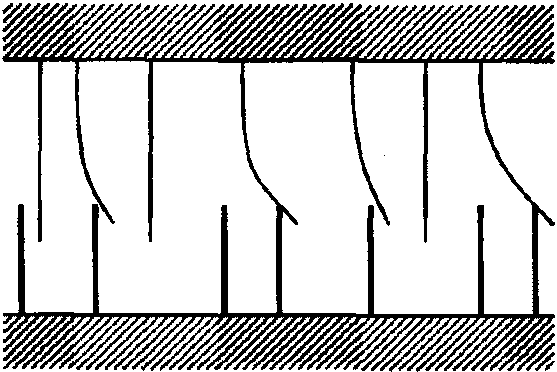
\includegraphics[width=0.75\textwidth]{bristles}
    \caption{Depiction of Dahl Model's Bristles \cite{p:dm}}
    \label{fig:bristles}
\end{figure}


% Dahl Model Math -----------------------------------------------------------
The Dahl model is defined as the following:
\begin{equation}
    F=F_{c}\left(1-e^{-\frac{ \sigma_{0}|x| }{ F_{c} }}\right)\mathrm{sgn}\left(\frac{\diff x}{\diff t}\right)
    \label{eq:dahlexp}
\end{equation}

Where $F_{c}$ is the coulomb friction of the surface, x is the displacement from original position (this is primarily focused on the microscopic displacements), and $\sigma_{0}$ is the "stiffness" of microscopic bumps and affects the shift to maximum coulomb friction.

To use this for state space equations we must find the derivative using chain rule:

\begin{align}
    \frac{\diff F}{\diff x} &= \cancel{-}\cancel{F_{c}}\cdot e^{-\frac{\sigma_{0}|x|}{F_{c}}}\cdot \cancel{-}\frac{\sigma_{0}}{\cancel{F_{c}}}\mathrm{sgn}\left(\frac{\diff x}{\diff t}\right)\mathrm{sgn}\left(x\right) \\
                            &= \sigma_{0}e^{-\frac{\sigma_{0}|x|}{F_{c}}}\mathrm{sgn}\left(\frac{\diff x}{\diff t}\right)\mathrm{sgn}\left(x\right)
\end{align}

\noindent
and to put the actual current force state back into this derivative function (since state space equations depend on previous states), we rearrange eq (1) to isolate $e^{-\frac{\sigma_{0}|x|}{F_{c}}}$ like such:

\begin{align}
    F&=F_{c}\left(1-e^{-\frac{ \sigma_{0}|x| }{ F_{c} }}\right)\mathrm{sgn}\left(\frac{\diff x}{\diff t}\right) \\
    \frac{F}{F_{c}} \mathrm{sgn}\left(\frac{\diff x}{\diff t}\right) &= 1-e^{-\frac{\sigma_{0}|x|}{F_{c}}} \\
    e^{-\frac{\sigma_{0}|x|}{F_{c}}} &= 1 - \frac{F}{F_{c}} \mathrm{sgn}\left(\frac{\diff x}{\diff t}\right)
\end{align}
and putting it back in the differential equation we get:

\begin{align}
    \frac{\diff F}{\diff x} &= \sigma_{0}\left(1-\frac{F}{F_{c}}\right)\cancel{\mathrm{sgn}\left(\frac{\diff x}{\diff t}\right)^{2}}\mathrm{sgn}\left(x\right) \\
    &=\sigma_{0}\left(1-\frac{F}{F_{c}}\right)\mathrm{sgn}\left(x\right)
\end{align}




The Dahl model's equation shares similar properties of an exponential function take of the stress-strain curve (depicted in figure \ref{fig:sscurve}), most notably, the point at which it shifts from an elastic spring to continual bristle movement

\begin{figure}[htbp]
    \center
    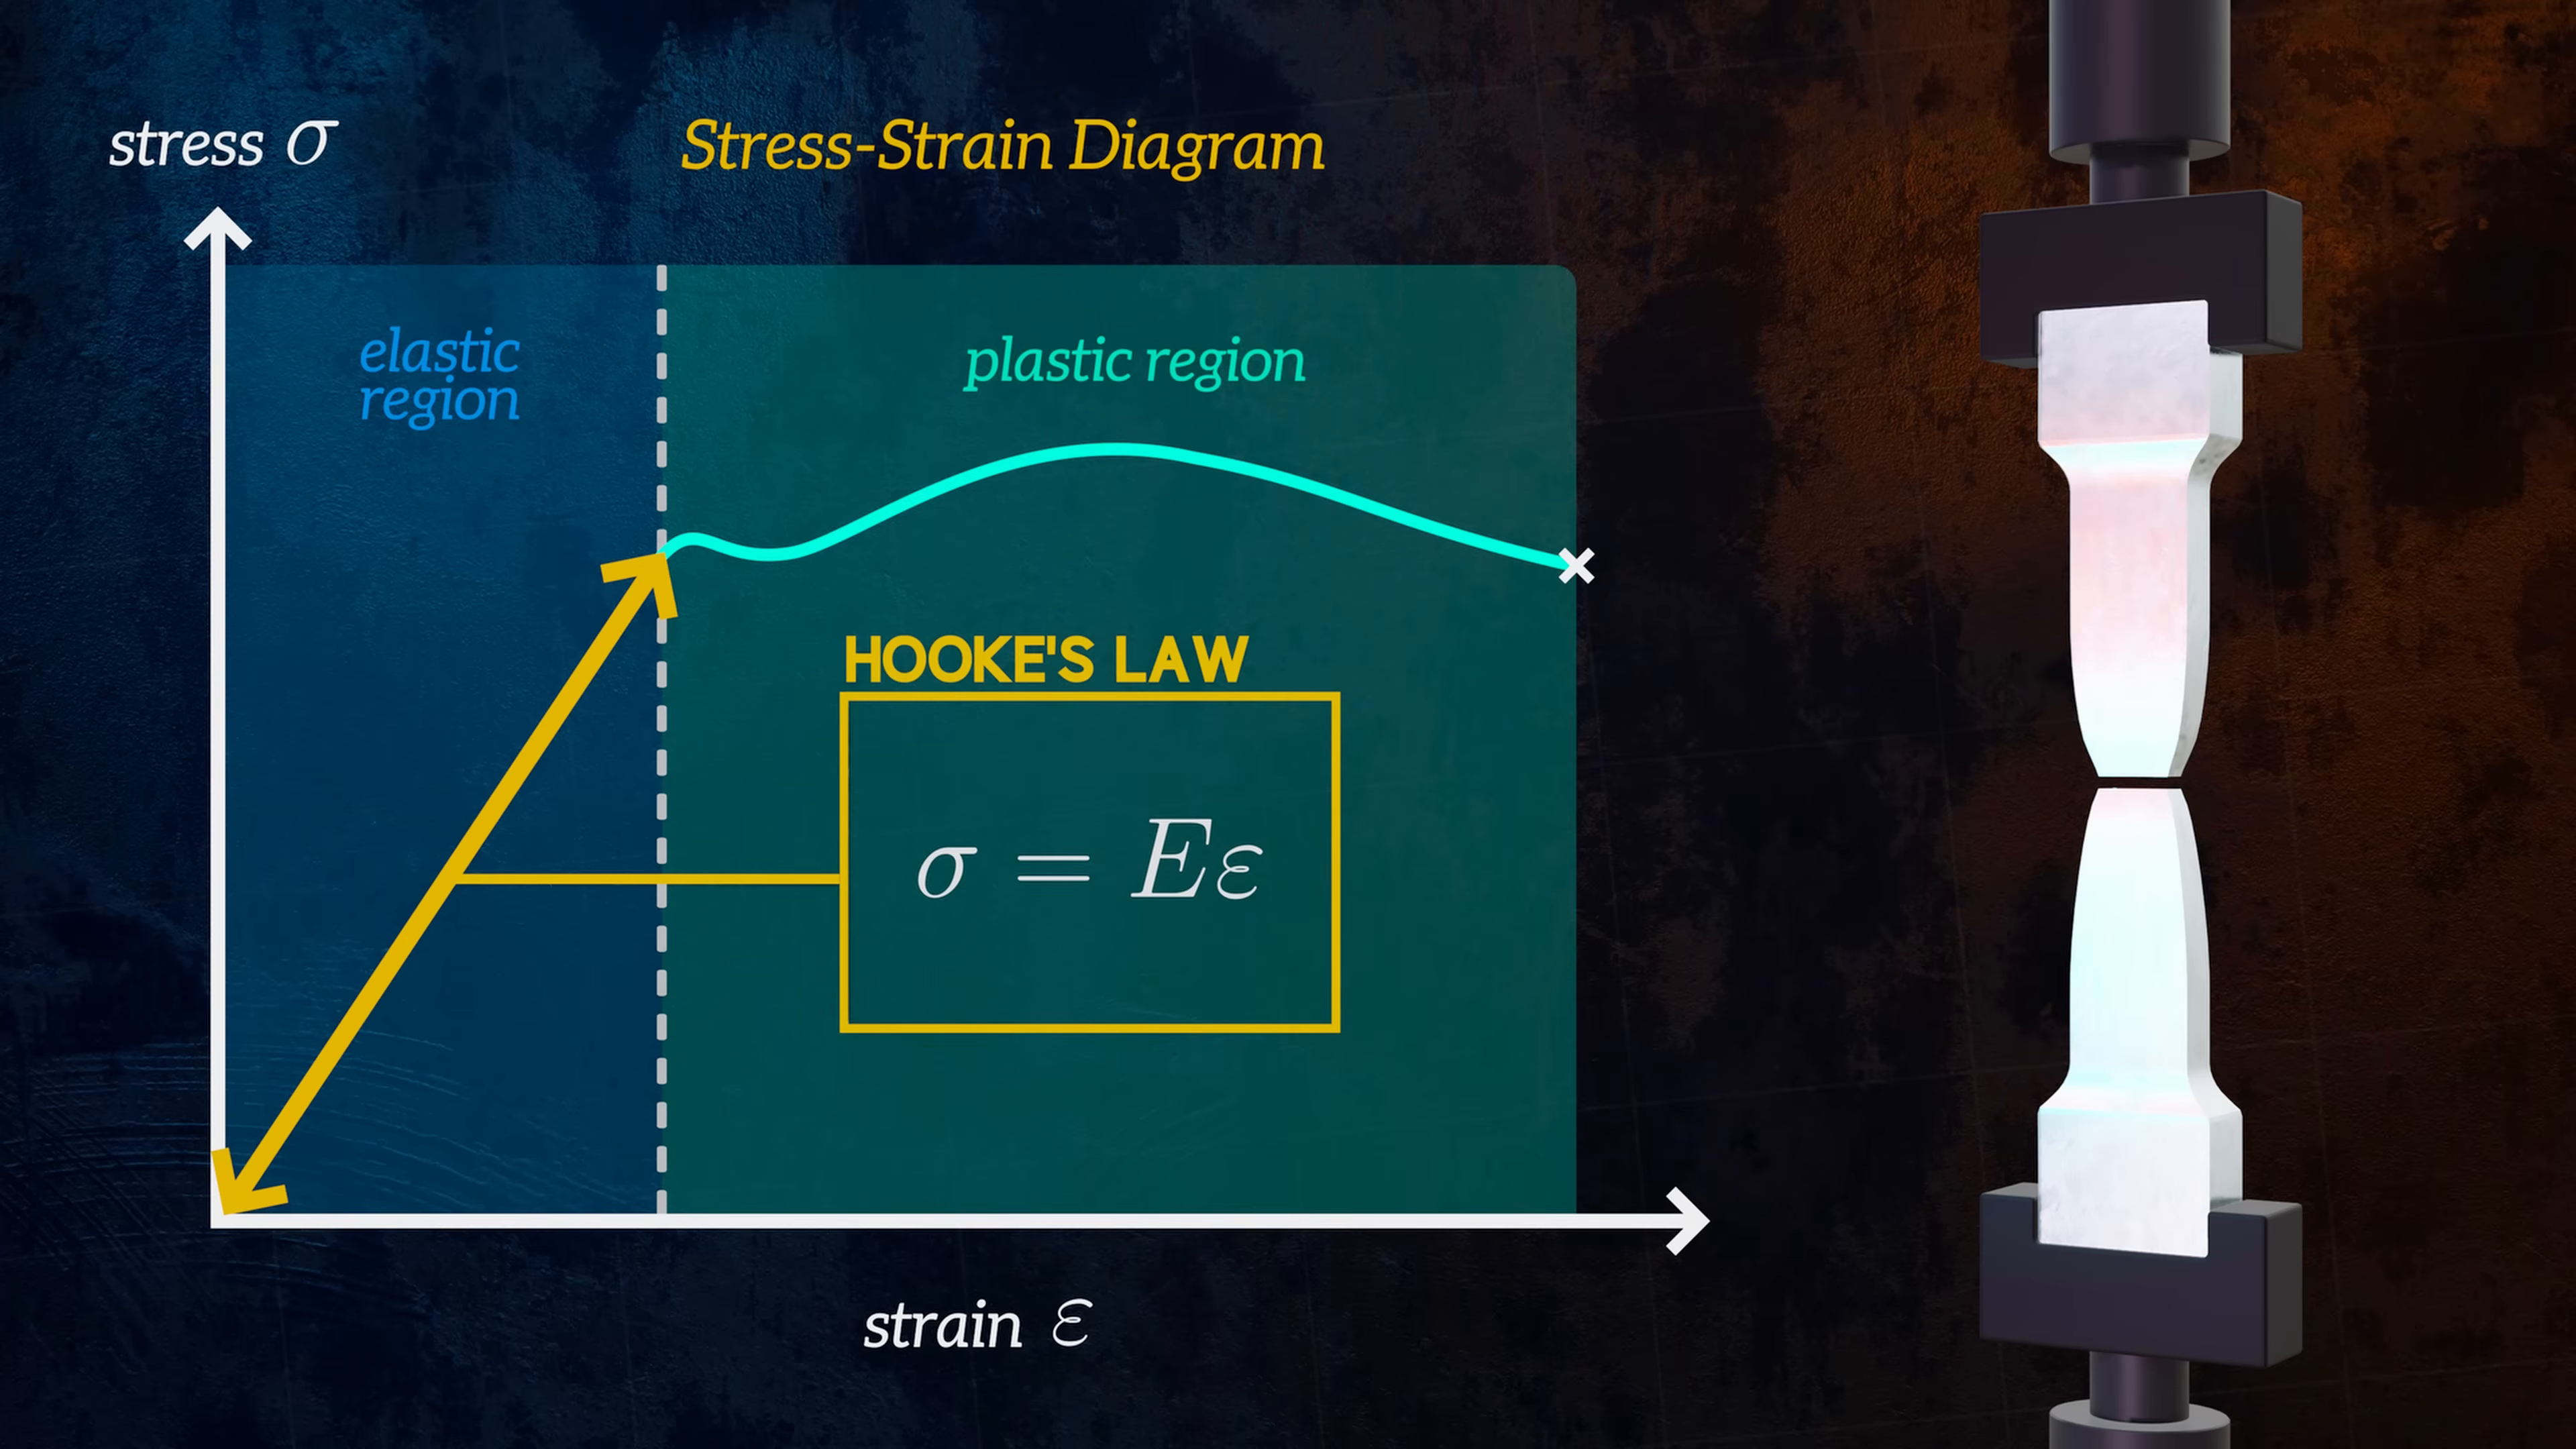
\includegraphics[width=0.7\textwidth]{stress strain curve}
    \caption{An annotation of a generic stress-strain curve\cite{youtube:sscurve}}
    \label{fig:sscurve}
\end{figure}
\begin{enumerate}
    \item Case 1: Current force = 0
        \begin{equation}
            \frac{\diff F}{\diff x} = 
        \end{equation}
\end{enumerate}


The labeled "elastic region" could be viewed as the predisplacement present in static friction before reaching the "plastic region" that is when it reaches coulomb friction.

\pagebreak

\pagebreak
\printbibliography
\end{document}
